%%%%%%%%%%%%%%%%%%%%%%%%%%%%%%%%%%%%%%%%%%%%%%%%%%%%%%%%%%%%%%%%%%%%%%%%%%%%%%%
%% 1.- ESTADO DEL ARTE
%%%%%%%%%%%%%%%%%%%%%%%%%%%%%%%%%%%%%%%%%%%%%%%%%%%%%%%%%%%%%%%%%%%%%%%%%%%%%%%

\cleardoublepage
\chapter{Estado del arte}
\chaptermark{Estado del arte}

\label{chap:estadoArte} % etiqueta para poder referenciar luego en el texto con ~\ref{sec:intro}
% \addcontentsline{toc}{chapter}{Introducción, Objetivos, Metodología y Planificación}

El presente proyecto parte de un pedido realizado por un cliente que pretende comunicar con kiconex los distintos equipos de un supermercado: muebles frigoríficos y máquinas de climatización. La mayoría de estos equipos dispone de un controlador propio, sin embargo, en el caso de la climatización, ha solicitado el diseño de un control a medida para el funcionamiento de una UTA. La instalación cuenta con los elementos de la \hyperref[figura:planoSupermercado]{Figura~\ref{figura:planoSupermercado}}:

\hspace{1em}

\begin{figure}[h]
  \centering
  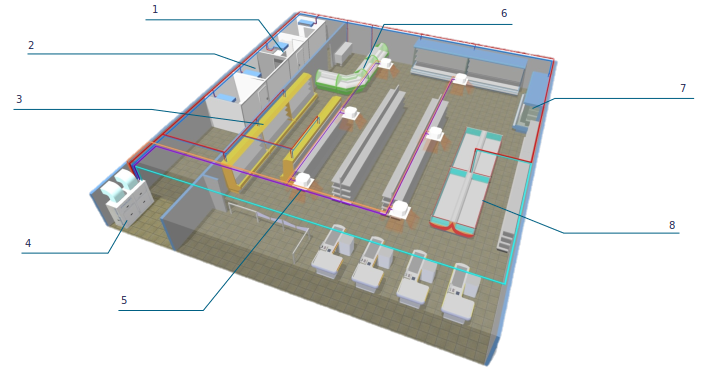
\includegraphics[width=16cm, keepaspectratio]{img/planoSupermercado}
  \caption{Plano de equipos del supermercado}
  \label{figura:planoSupermercado}
\end{figure}

\begin{enumerate}
  \item Obradores.
  \item Cámaras frigoríficas.
  \item Murales de lácteos.
  \item Bomba de calor.
  \item Unidades de Tratamiento de Aire.
  \item Vitrinas expositoras.
  \item Semimurales de carne, frutas y verduras.
  \item Islas de congelados.
\end{enumerate}

Kiconex emplea en sus desarrollos controladores de Dixell\footnote{\url{https://climate.emerson.com/es-es/brands/dixell}}, en concreto los modelos \textit{IPG208} e \textit{IPG215} de \textit{iPro}\footnote{\url{https://climate.emerson.com/documents/ipro-series-en-4923358.pdf}}, con los módulos de expansión IPX206 e IPX215\footnotemark[2]. El modelo a emplear dependerá de las especificaciones de entradas y salidas de la UTA que aparece en la \hyperref[figura:planoSupermercado]{Figura~\ref{figura:planoSupermercado}}. A continuación, en el \hyperref[sec:kiconex]{apartado 1 de este capítulo} se describe el software necesario para la programación de un control de este tipo.

El dispositivo inalámbrico a diseñar, mencionado en el \hyperref[chap:intro]{apartado de introducción anterior} comunicará los muebles frigoríficos: Murales de lácteos, vitrinas expositoras, semimurales e islas de congelados. El hardware empleado, descrito en el \hyperref[sec:esp32poe]{apartado 3 de este capítulo}, se basa en el chip ESP32\footnote{\url{https://www.espressif.com/en/products/socs/esp32/overview}}. Para entender el papel de este dispositivo en la red, es necesario conocer el funcionamiento de una instalación desde el punto de vista de kiconex, atendiendo a cómo se integra cada elemento. El \hyperref[sec:kiconex]{apartado 2 de este capítulo} se dedica por completo a describir la estructura de un sistema basado en kiconex.

\section{iPro y su pantalla}
\label{sec:iproypantalla}

\begin{figure}[h]
  \centering
  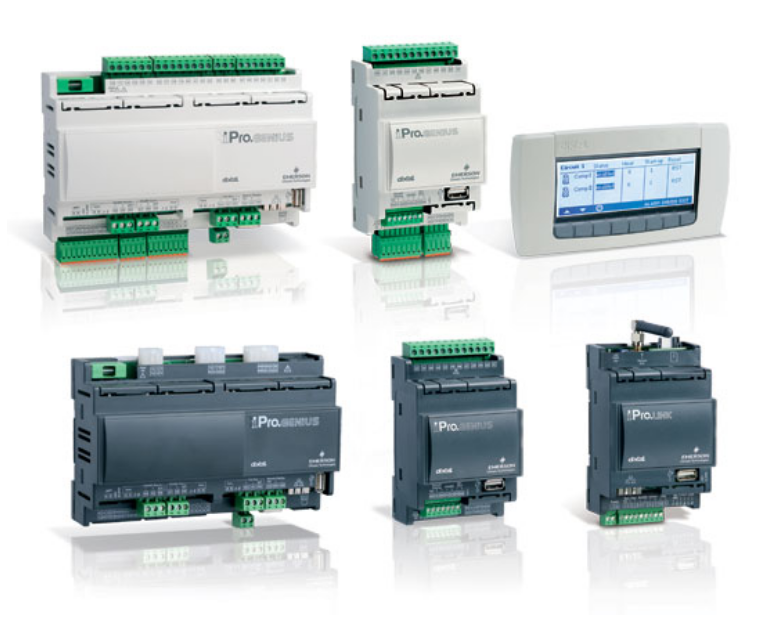
\includegraphics[width=12cm, keepaspectratio]{img/iproSeries}
  \caption{iPro Series}
  \label{figura:iproSeries}
\end{figure}

\textit{iPro} (\hyperref[figura:iproSeries]{Figura~\ref{figura:iproSeries}}) es la gama de controladores programables ofrecida por Dixell. La gama consta de controladores programables, ampliaciones de E/S, controladores para válvulas electrónicas e interfaces gráficas adaptadas para cubrir cualquier tipo de aplicación en el sector del aire acondicionado, el sector de la refrigeración y cualquier área relativa. Algunas de sus especificaciones son:

\begin{itemize}
  \item Alimentación a 24Vac/dc.
  \item Microprocesador ARM9 de 32 bits (200MHz).
  \item El programa y los parámetros se almacenan en una memoria flash permanente. No se pierden datos en caso de fallo de alimentación.
  \item Servidor web interno.
  \item Hasta 80 Mb de memoria flash, dependiendo del modelo.
  \item Entradas y salidas completamente configurables.
  \item Conexiones:
  \begin{itemize}
    \item Puerto Ethernet.
    \item Puerto USB.
    \item Conexión dedicada para un display LCD.
    \item CANBus.
    \item RS485 Master.
    \item RS485 Slave.
  \end{itemize}
\end{itemize}

Los modelos se diferencian en el tamaño (10 DIN o 4 DIN) y en el número de entradas y salidas (analógicas y digitales). La \hyperref[tab:esipro]{Tabla~\ref{tab:esipro}} recoge las especificaciones de los modelos empleados por kiconex.

\begin{table}[h]
  %\centering
  \begin{center}
    \setlength\arrayrulewidth{2pt}
    \begin{tabular}{ r | c !{\vrule width 0.25pt} c | c !{\vrule width 0.25pt} c | }
      %\Cline{2pt}{2-5}
      \hhline{*{1}{~}|*{4}{-}}
      \multirow{2}{*} & \multicolumn{2}{c|}{\cellcolor{lightgray}Controlador} & \multicolumn{2}{c|}{\cellcolor{lightgray}Módulo de Expansión}   \\ \Cline{0.25pt}{2-5}
      & \textbf{IPG208} & \textbf{IPG215} & \textbf{IPX206} & \textbf{IPX215} \\ \cline{1-1} \Cline{0.25pt}{2-5}
      \multicolumn{1}{|r|}{\textbf{Entradas analógicas}} & 6 & 10 & 7 & 10 \\
      \multicolumn{1}{|r|}{\textbf{Salidas analógicas}} & 4 & 6 & 3 & 6 \\
      \multicolumn{1}{|r|}{\textbf{Entradas digitales}} & 11 & 20 & 3 & 20 \\
      \multicolumn{1}{|r|}{\textbf{Salidas digitales (Relés)}} & 8 & 6 & 8 & 15 \\ 
      \noalign{\hrule height 2pt}
    \end{tabular}
    \caption{Especificaciones de E/S para distintos modelos de iPro.}
    \label{tab:esipro}
  \end{center}
\end{table} 

Dixell dispone de dos modelos de displays compatibles con el \textit{iPro}: \textit{VGIPG} y \textit{VTIPG}\footnote{\url{https://climate.emerson.com/es-es/shop/1/dixell-electronics-sku-vtipg-hmi-es-es}}. Para el diseño de dichas pantallas, se emplea el software \textit{Visoprog}\footnote{\url{https://climate.emerson.com/es-es/shop/1/dixell-electronics-sku-visoprog-es-es}} de Dixell, que importa las variables creadas en la programación del controlador, para poder configurar en la pantalla la interacción con las mismas. 

\subsection{Programación iPro}
\label{subsec:iproprog}

Para la programación del \textit{iPro} se emplea el software \textit{ISaGRAF}\footnote{\url{https://www.logicbus.com.mx/isagraf.php}}, ya que ofrece un entorno de desarrollo estándar e internacional, soportando varios lenguajes de programación diferentes según las normas IEC61131. Se trata de un software usado en todo el mundo y que también permite simular el sistema programado. Los estándares de programación soportados son:

\begin{itemize}
  \item (\textbf{LD}) Escalera  
  \item (\textbf{FBD}) Diagrama a Bloques 
  \item (\textbf{SFC}) Tabla de Funciones Secuenciales 
  \item (\textbf{ST}) Texto Estructurado 
  \item (\textbf{IL}) Lista de Instrucciones 
  \item (\textbf{FC}) Diagrama de flujo 
\end{itemize}

Para comenzar a realizar un programa se parte de una plantilla ya preparada previamente por kiconex para configurar entradas, salidas, parámetros, alarmas, avisos, etc.. Es por ello que primero es necesario conocer las especificaciones del sistema a programar. La Figura xxx representa un ejemplo de configuración de entradas analógicas. Como se puede ver, hay un vector que representa las entradas, y para cada una de ellas se especifica la configuración posible y el uso destinado.

XXX-FIGURAPROGRAMA

A cada variable de parámetro, alarma, aviso, estado y entradas/salidas se le asigna una dirección de registro, como se puede ver en la Figura xxx. Lo habitual es destinar distintos rangos de direcciones a cada tipo de variable.

XXX-FIGURATABLAREGISTROS

\subsection{Configuración de la pantalla}
\label{subsec:displayconfig}

Para la configuración de la pantalla, se emplea \textit{Visoprog}, un software ofrecido por la misma marca Dixell, especialmente para su uso con los modelos \textit{VGIPG} e \textit{VTIPG}. En este caso también se ha partido de una plantilla previamente preparada por kiconex con las distintas pantallas que necesita un control como el \textit{iPro}:

\begin{itemize}
  \item pantalla1  
  \item pantalla1 
  \item pantalla1
  \item pantalla1 
  \item pantalla1 
  \item pantalla1 
\end{itemize}

Para usar este programa, en primer lugar se importa un fichero de registros generados por \textit{ISaGRAF}. Así es como \textit{Visoprog} los conoce y permite que el usuario interactúe con los mismos en el proceso de navegación por la pantalla, habiendo configurado previamente dicha interacción.

\textit{Visoprog} tiene también una sección destinada a textos estándar, así se puede cambiar un texto en un solo sitio, y no en los cincuenta sitios en los que se está empleando. La Figura xxx representa el aspecto de la interfaz del programa.

XXX-FIGURAVISOPROG

\section{Kiconex}
\label{sec:kiconex}

Como ya se ha mencionado en la \hyperref[chap:intro]{introducción}, kiconex es una plataforma de supervisión y control para equipos de climatización y frío industrial. Entre sus funciones se encuentra:
\begin{itemize}
  \item \textbf{Almacenamiento en la nube} de datos de temperatura, estado de funcionamiento, presiones, etc.  
  \item \textbf{Gráficas} para visualizar la evolución de los datos en el tiempo, permitiendo compararlos. 
  \item \textbf{Control remoto}: marcha/paro, cambio de consigna, etc.
  \item \textbf{Reglas} con programaciones horarias o acciones frente a condiciones. 
  \item \textbf{Diagramas} para introducir un plano del edificio y sobre ese plano ver la temperatura de las salas y, por ejemplo, encender y apagar.
  \item \textbf{Alarmas} con posibilidad recibir alertas en caso de fallo del equipo. 
\end{itemize}
Para su funcionamiento, kiconex se compone de los siguiente elementos:
\begin{enumerate}
  \item \textbf{Servidor en la nube}, donde se almacenan los datos.
  \item \textbf{Plataforma de visualización y control}.  
  \item \textbf{Kibox}: hardware que actúa como pasarela entre la nube y el equipo de frío o clima. Recibe mensajes de la nube a través de MQTT, los procesa y los envía en formato Modbus al equipo final. Este último, recibe el mensaje, lo procesa y envía una respuesta que sigue el camino inverso hasta que la nube recibe el dato solicitado. 
  \item \textbf{Equipos} de climatización o frío industrial: emplean el estándar industrial Modbus. La mayoría emplean Modbus RTU pero kiconex también funciona a través de Modbus TCP. Estos equipos reciben los mensajes del \textit{kibox} y le envían una respuesta.
  \item \textbf{Kiwi}: aún no está en venta, ya que se trata del dispositivo inalámbrico que se ha desarrollado en este proyecto, pero el objetivo es su actuación como esclavo Modbus, recibiendo mensajes del maestro \textit{kibox} a través de TCP-IP. \textit{Kiwi} retransmite estos mensajes actuando como maestro, a los dispositivos de frío y clima (esclavos). Es decir, \textit{kiwi} es un maestro-esclavo: maestro de cara a los equipos y esclavo de cara al \textit{kibox}.
\end{enumerate}

xxx-figuraredkiconex

La plataforma de supervisión, para poder comunicarse con los controles de los equipos de frío y clima, necesita conocer sus registros. Para ello, en la plataforma existe un apartado llamado "librerías", en el cual se pueden ver y crear los mapeados de registros de los controles que se necesiten. En la Figura xxx se puede ver el aspecto de una librería en la plataforma.

xxx-figuralibreria

Para el caso del \textit{iPro}, en el cual el programa se diseña desde cero por kiconex, el mapeado de registros se extrae directamente del software \textit{ISaGRAF}, y se introduce en una nueva librería en la plataforma. Cuando se trata de otros controles, es el cliente quien lo consigue a través del fabricante. kiconex, gracias a su trayectoria, ya ha recopilado una gran cantidad de librerías para multitud de controles, lo que facilita mucho el proceso.

\section{ESP32-PoE}
\label{sec:esp32poe}

xxx-placaesp32

El hardware empleado para el desarrollo del kiconex inalámbrico (\textit{kiwi}) se basa en el chip ESP32 xxx. El modelo empleado es el Olimex ESP32-PoE (Figura xxx). Olimex xxx es una empresa de Bulgaria líder en fabricación electrónica para el mercado integrado. Su modelo ESP32-PoE ha sido elegido por disponer de un puerto UEXT desde el que se puede obtener una interfaz RS-485 a través de un conversor, para la comunicación a través de Modbus RTU. También dispone de puerto ethernet que puede usarse bien como conexión a internet vía ethernet o bien para conectar un equipo por modbus TCP.

xxx-conversoruext

La Figura xxx representa los pines de entrada y salida de la placa y del conector UEXT:

xxx-pines

Para la elaboración del código de programación del kiwi, se va a aprovechar parte del código empleado en las siguientes librerías ya existentes en github xxx:

\begin{itemize}
  \item Librería Modbus RTU  
  \item Librería Modbus TCP 
  \item Librería WiFiManager
\end{itemize}

%%%%%%%%%%%%%%%%%%%%%%%%%%%%%%%%%%%%%%%%%%%%%%%%%%%%%%%%%%%%%%%%%%%%%%%%%%%%%%%
%%%%%%%%%%%%%%%%%%%%%%%%%%%%%%%%%%%%%%%%%%%%%%%%%%%%%%%%%%%%%%%%%%%%%%%%%%%%%%%
%%%%%%%%%%%%%%%%%%%%%%%%%%%%%%%%%%%%%%%%%%%%%%%%%%%%%%%%%%%%%%%%%%%%%%%%%%%%%%%
